\newcommand{\upcite}[1]{\textsuperscript{\textsuperscript{\cite{#1}}}}
\chapter{绪论}
\section{背景与意义}

根据原始神经元图像信息的神经元追踪和数字重建是神经科学界热门方向。神经元的形态反应出它的功能,相同功能的神经元通常具有类似的功能。神经科学家通过结构脑图谱的重建,可以反推大脑是如何运作,对理解智慧的产生有重要的帮助。十九世纪以来,神经科学家们开始推测记忆,甚至个性与智力都和大脑神经元之间的连接有密切的联系。图 \ref{worm} 展示了秀丽隐杆线虫的神经结构的神经结构,图中每一个节点均代表一个神经元,每一条线代表一个连接。它仅仅由 300 个神经元组成,之间的连接也仅有 7000 个。

\begin{figure}
\centering
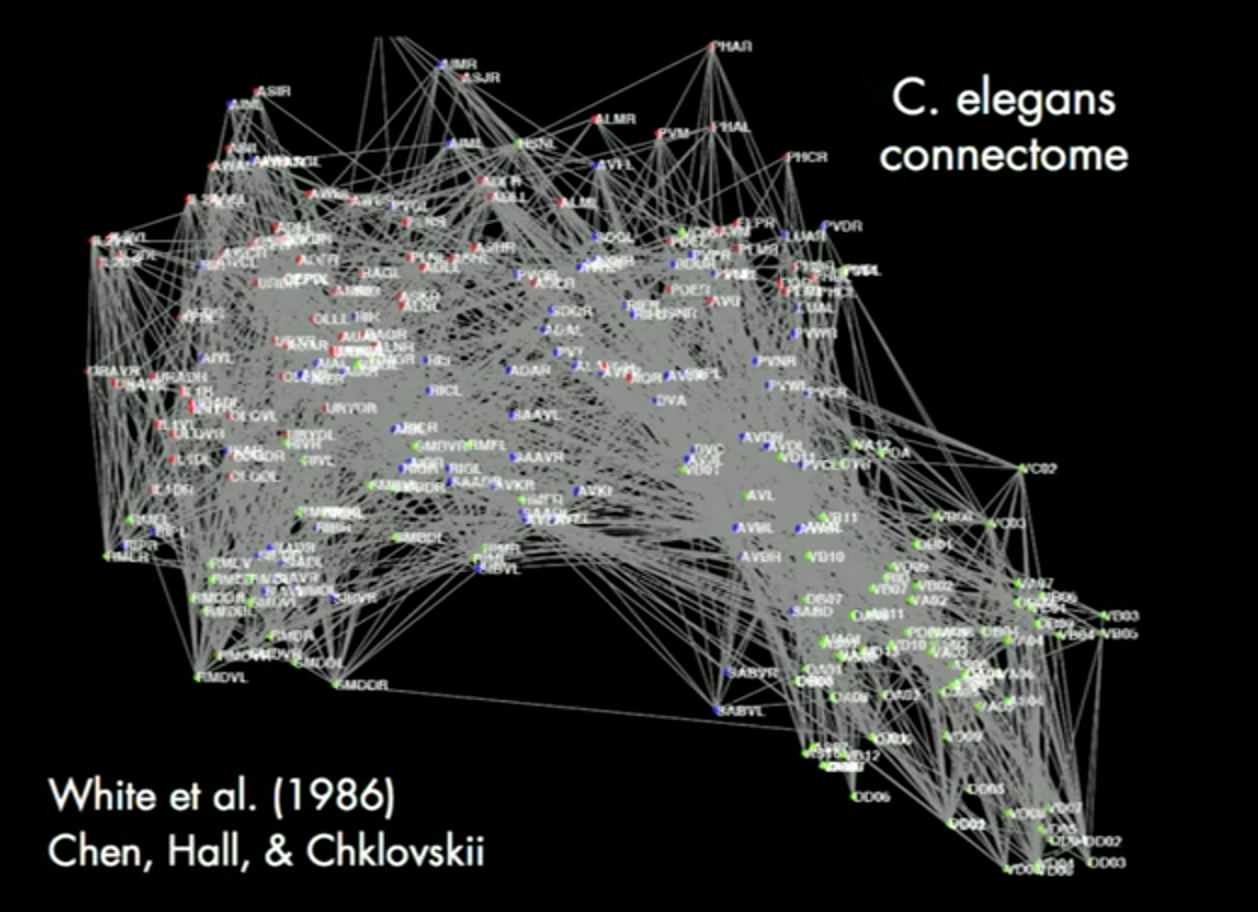
\includegraphics[width=108mm]{images/worm}
\caption{秀丽隐杆线虫的神经结构,其中的点代表了一个神经元结构并标注了相应的名称,线将神经元连接起来,表明对应的神经元通过神经纤维建立了联系}
\label{worm}
\end{figure}

White, John G 与 Southgate 等人在 1986 年时已经 利用一系列局部原始电子显微照片对秀丽隐杆线虫的神经系统的进行了完整重建\upcite{white1986structure}。经过了 30 多年的发展,Yunkyu Sohn,Myung-Kyu Choi 与 Yong-Yeol Ahn 等人于 2011 年利用基于模块化的群态检测算法发现秀丽隐杆线虫中包含了 5 个解剖簇及其对应的实验可识别功能电路,进一步揭示了生物电路如何产生更高阶的复杂行为\upcite{varshney2011structural}。即使如此,由于神经网络复杂的拓扑结构,神经科学家们仍旧未能充分探索仅仅由 300 个神经元通过突触交织而成的神经网络结构。而人类大脑由一千亿个神经元组成,神经元之间连接的数量又是神经元数量的一万倍,远比秀丽隐杆线虫的神经结构要复杂的多。因此,设计并实现自动神经元重建算法便成了探索神经结构的重要步骤之一。

Druckmann, Shaul 与 Feng 等人开发的神经元重建算法提供了准确的中线,直径,表面,体积和分支点位置,支持沿着神经元表面分析标记过的分子分布,还可以直接导出到建模软件\upcite{druckmann2014structured}。图 \ref{Druckmann} 展示了这种神经元重建算法的样例结果。Brown, Kerry M 与 Barrionuevo 等人收集了来自不同动物,脑区,神经元类型和可视化方法的六个数据集,为自动化软件所需的测试提供了基准,提高了重建的质量,同时最大限度地减少了人工的参与,极大的促进了神经元重建领域的发展\upcite{brown2011diadem}。

\begin{figure}
\centering
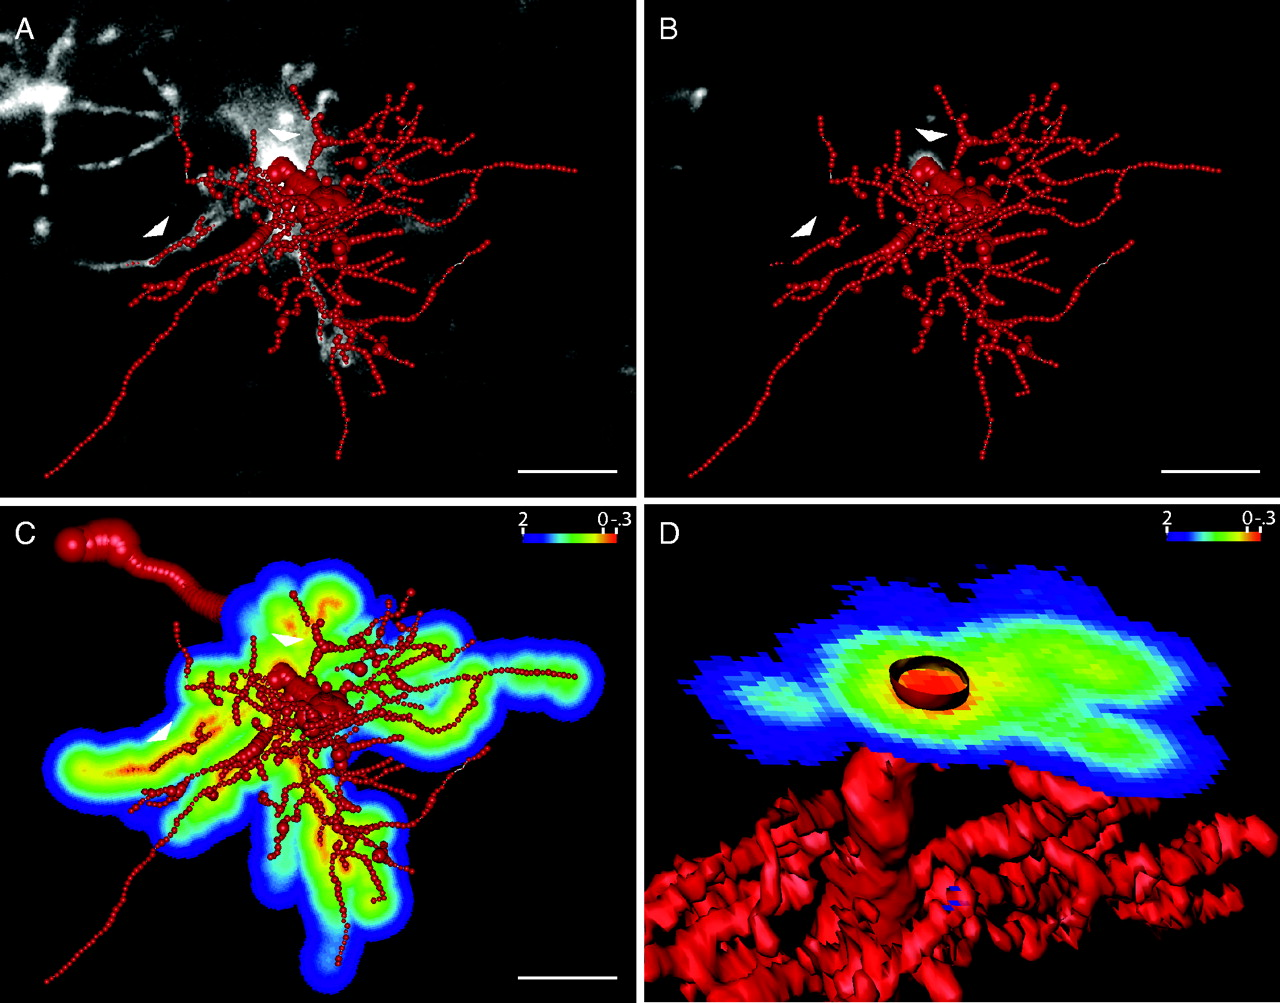
\includegraphics[width=108mm]{images/Druckmann}
\caption{Druckmann 等人的神经元重建算法的样例结果 白色的是原始神经元图像,红色的表示完成重建的神经元结构,蓝色和绿色表示对应神经元的表面概率}
\label{Druckmann}
\end{figure}

由于神经元拓扑结构的复杂性,在一些自动化重建结果的细节上仍然需要研究人员对数字重建的结果进行人工纠正和修改,以确保数字重建工作的准确性。另外研究人员需要对数字重建结果进行编辑,比如添加或删除一些网络分支等。为了便于研究人员进一步研究神经结构,探索智能产生的原因,这就需要在神经元自动重建算法的基础上建立交互式神经元重建系统,进一步提升数字重建结果的准确性,并且将多部分数字重建结果合并起来。

\section{现有系统的特点与问题}
\subsection{FARSIGHT}
FARSIGHT 的软件界面如图 \ref{FARSIGHT} 所示,图中正在编辑的是一小段神经结构,展示了用户点击位置,根节点方向,以及分支节点。
\begin{figure}
\centering
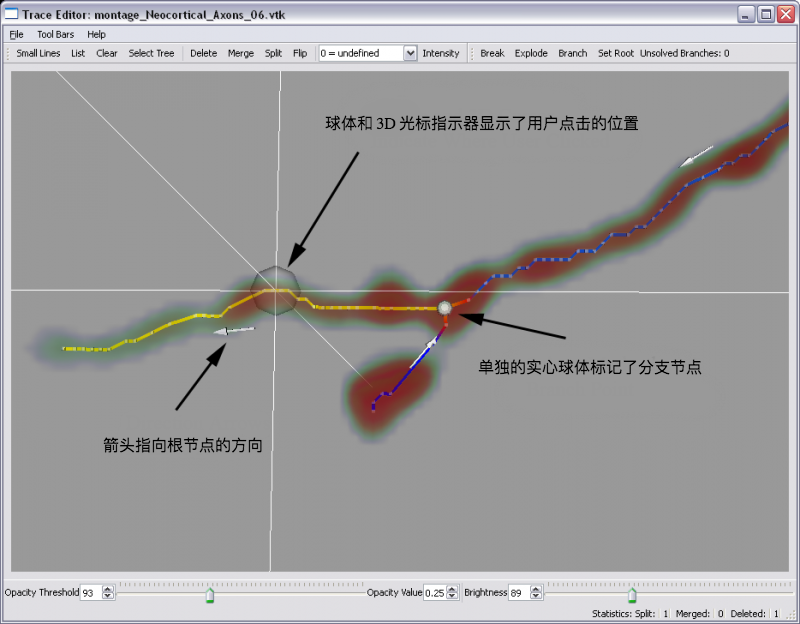
\includegraphics[width=108mm]{images/FARSIGHT}
\caption{FARSIGHT 软件运行界面 箭头指向根节点的方向,单独的实心球标记了分支节点,球体和 3D 光标指示器显示了用户点击的位置}
\label{FARSIGHT}
\end{figure}

FARSIGHT 的设计目标是保证重建结果的细节,可以快速识别重建结果的错误并能迅速纠正。FARSIGHT 利用基于模式分析辅助集群编辑(PACE)的思想,根据对自动跟踪结果的定量测量和多变量模式分析工具的分析结果,发现其中常见类型的重建错误,提高纠正重建结果的效率\upcite{luisi2011farsight}。图 \ref{FARSIGHT-res} 展示了 FARSIGHT 导出的较大规模的神经结构重建结果。

\begin{figure}
\centering
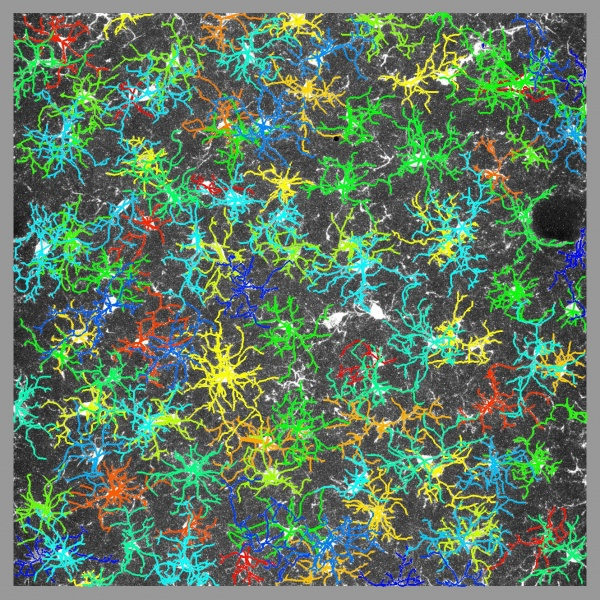
\includegraphics[width=108mm]{images/FARSIGHT-res}
\caption{FARSIGHT 导出的重建结果 每种颜色均代表了一部分神经结构}
\label{FARSIGHT-res}
\end{figure}

FARSIGHT 的缺点在于,它专注于半自动重建,对于常见的错误修改效率确实较高,但是如果遇到细小的错误,FARSIGHT 无法识别,也不提供精细化的编辑手段,需要借助于其他软件完成。

\subsection{neuTube}
neuTube 是一种基于 SWC 文件格式的神经元重建软件,同时具备 2D 和 3D 的可视化以及直观地编辑、绘制功能,允许用户高效的根据荧光图像数据重建神经元结构,并且支持编辑其他软件生成的标准神经结构的文件\upcite{Feng2014neuTube}。软件界面如图 \ref{neutube} 所示。

\begin{figure}
\centering
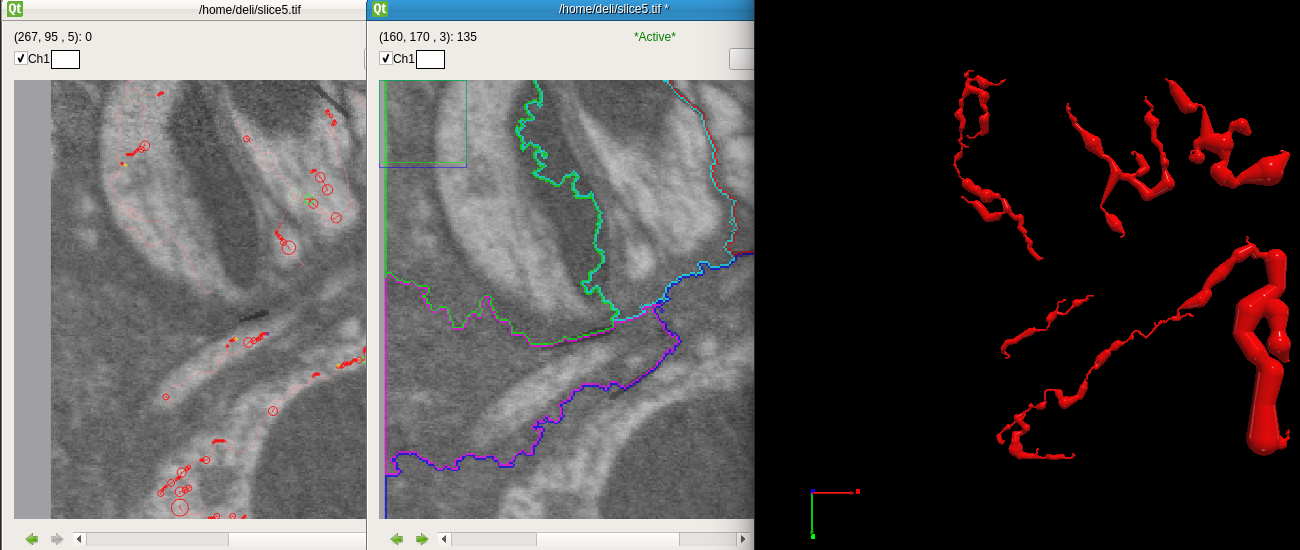
\includegraphics[width=108mm]{images/neutube}
\caption{neuTube 软件运行界面 图中展示了神经元自动重建与编辑的过程,第一个界面中红色的点是随机产生的种子点,第二个界面是根据种子点对神经元结构进行分割,图三是完成重建的神经元结构并支持用户进行纠错、编辑}
\label{neutube}
\end{figure}

虽然 neuTube 提供了 2D 和 3D 模式下精细编辑神经结构的功能,但是无法进行多人协同编辑,无法分享完成重建的结构脑胞体。

通过分析不难看出,现有的软件难以支持多名神经科学家同时进行精细化的神经结构编辑。由于神经结构的复杂性,团队合作进行神经结构的编辑,结果合并等是未来神经科学发展的趋势,因此需要设计并开发一个支持多用户协同工作的在线交互式神经元编辑平台便显得尤为重要。

\section{论文结构}
本文旨在设计并实现在线多用户的神经元网络结构编辑分享平台,利用互联网便于数据共享与交流的特点解决一些现有神经元编辑软件的问题,使得神经科学家可以便捷地进行异地,多用户协同编辑神经元网络结构,并能分享完成重建的结构脑图谱,探索神经元结构下的奥秘。由于项目涉及到数据可视化与后台服务器搭建,自然地将整个项目分成两部分,这里主要实现后台服务器的搭建,为前端可视化操作提供了有力的支持。

第一章讨论了交互式神经元重建系统的背景与意义以及现有的神经元编辑软件存在的问题,第二章讨论了项目整体架构并简单介绍所用到的技术
。第三章讨论技术实现的细节以及如何根据性能测试结果进行性能优化,第四章描述了在性能优化之后的系统整体性能,第五章讨论了接下来的工作并分析了项目中存在的不足。

